\documentclass[12pt]{report}
\usepackage{graphicx}
\usepackage{color}

\begin{document}
\chapter{Contribution}
\begin{center}
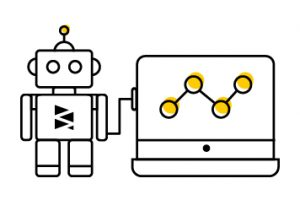
\includegraphics[width=300]{Machina.jpg}

\end{center}
\newpage
\section{Introduction}
Dans ce chapitre, nous abordons le dernier volet de ce mémoire, qui a pour objectif l'exposition de la phase de réalisation de notre projet. Cette phase est considérée comme étant la concrétisation finale de notre recherche représentée par le développement et l'évaluation d'un modèle de prédiction, de l'activité biologique et finalement d'un ensemble de molécules par l'apprentissage en profondeur. Tout d'abord, nous allons expliqué la démarche et la méthode proposée, ensuite nous détaillons l'implémentation de l'approche proposée ainsi que les outils utilisés pour illustrer le fonctionnement du modèle. Enfin, nous discutons les résultats obtenus par notre modèle et les comparer avec d'autres approches dans la littérature.    

\section{Description de la méthode proposée}
Maintenant, nous allons fait le point pour expliquer notre démarche quant va utilisé pour ce faire notre projet  et qui va nous permettre de mettre en pratique , avec suggères les étapes suivantes :\\
\begin{enumerate}
\item Importer les bibliothèque quand va utilisé
\item La lecture des données à partir le fichier csv de dataset
\item La transformation de données word2vect
\item Définie le modèle avec leur architecture 
\item Mettre le modèle à l'entrainement sur les données
\item L'évaluation de modèle avec le test
\item La prédiction des valeur 
\end{enumerate}
\newpage
\section{Schéma de la méthode proposé}
\begin{figure}[h]
\begin{center}
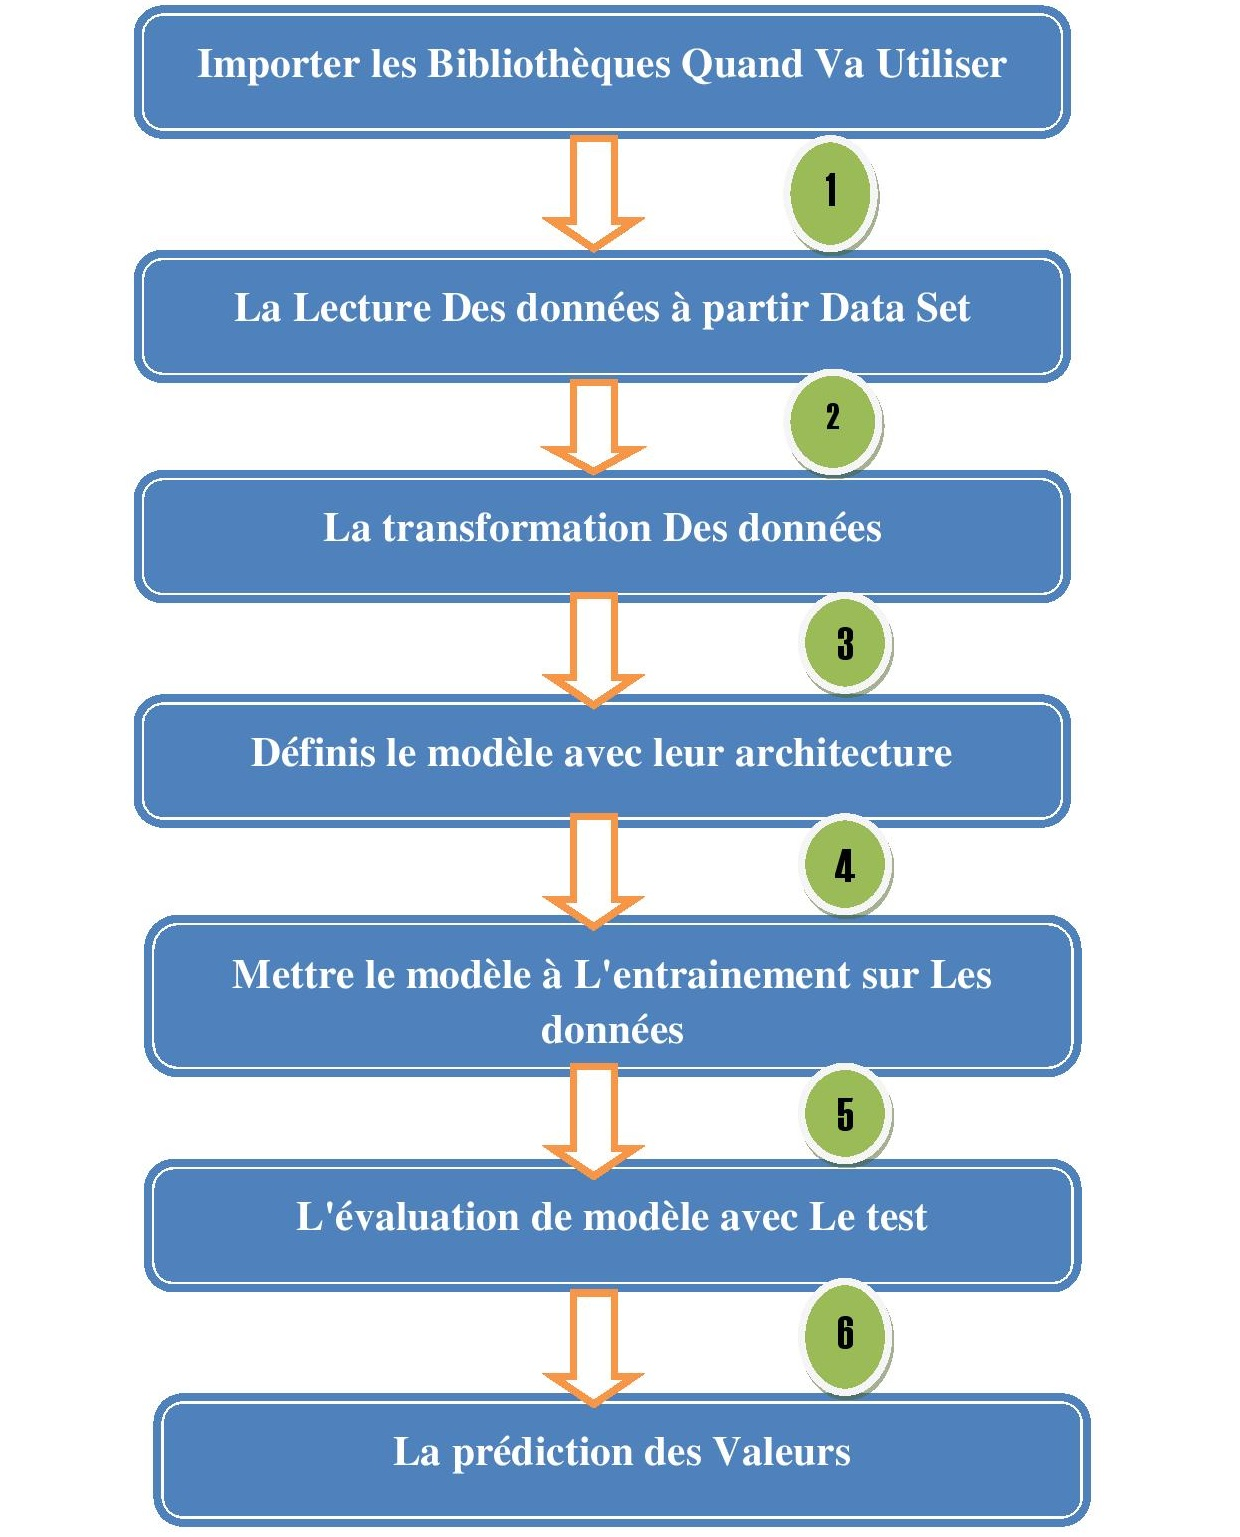
\includegraphics[width=300]{demarche.jpg}
\caption{Les étapes de la méthode proposé}
\end{center}
\end{figure}




\newpage 
\subsection{Différence entre le développement traditionnel et l'apprentissage automatique }
Le diagramme suivant illustre la différence entre l'apprentissage automatique et le développement de logiciel traditionnel \cite{ref25} :
\begin{figure}[h]
\begin{center}
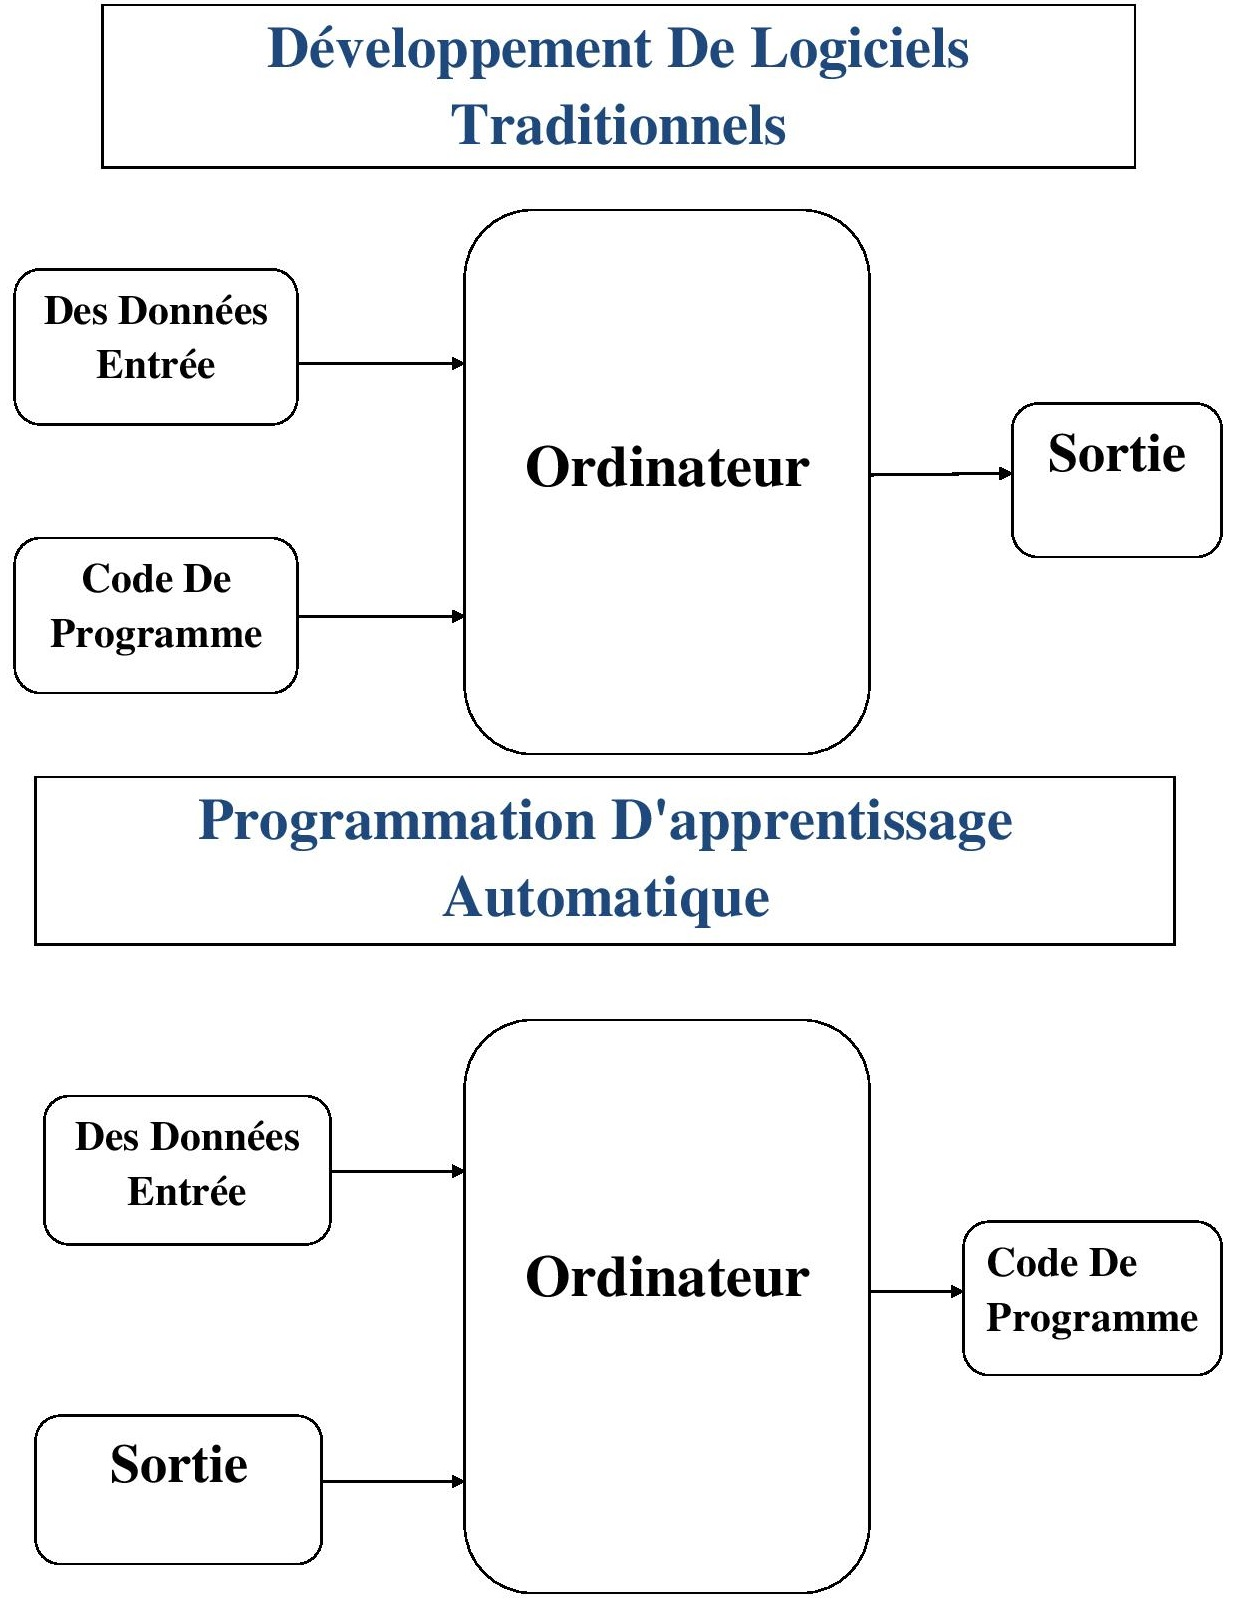
\includegraphics[width=250]{jkjk.jpg}
\caption{le développement traditionnel et l'apprentissage automatique}
\end{center}
\end{figure}

\subsubsection{Développement de logiciel traditionnel}
Les programmeurs créent des programmes qui spécifient comment transformer une entrée en sortie souhaitée \cite{ref25} .
\subsubsection{L'apprentissage automatique}
Les programmeurs créent des modèles qui peuvent apprendre à produire la sortie souhaitée pour une entrée donnée. Cet apprentissage remplit le rôle traditionnel du programme informatique \cite{ref25} .
\subsection{Le langage de programmation choisir}
C'est bien beau de vouloir apprendre un langage de programmation, mais il faut savoir lequel choisir. alors pour notre projet nous allons utiliser le langages \textbf{python} .
\begin{figure}[h]
\begin{center}
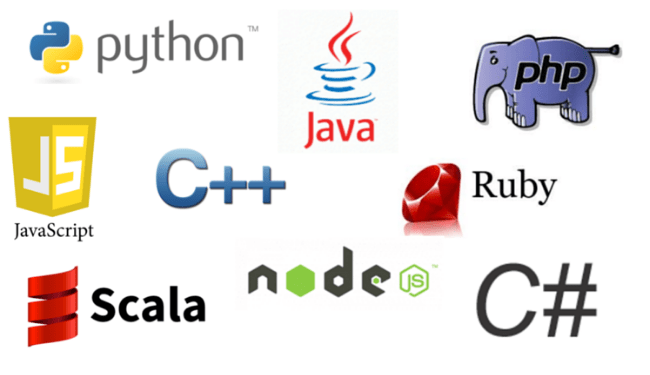
\includegraphics[width=300]{cchoil.png}
\caption{Langages de programmation}
\end{center}

\end{figure}

\subsection{Python}
\begin{multicols}

\includegraphics[width=50]{python.png}
python est un langage de programmation open source interprété côté serveur et non compilé. Créé par Guido van Rossum \cite{ref24}, il est utilisé pour le développement web, le développement de jeux-vidéos et autres logiciels, ainsi que pour les interfaces utilisateur graphiques. Il a notamment été utilisé dans la création d'Instagram, de YouTube et de Spotify, et est l'un des langages de programmation officiels de Google.
\end{multicols}


\subsection{Pour quoi nous choisir le python}
au niveau de notre projet qui représente python est le langage de programmation le plus utilisé dans le domaine du Apprentissage en profondeur et de la Data Science. qui fournit des bibliothèque très puissante. qui permettent de coder des algorithmes d'intelligence artificielle et de machine learning, en particulier des réseaux de neurones .


\subsection{Les bibliothèques}
Avant de commencer à attaquer notre script nous avons beaucoup de  \textbf{bibliothèques}  qui nous permettent et nous aident à travailler pour implémenter ce modèle .
\begin{figure}[h]
\begin{center}
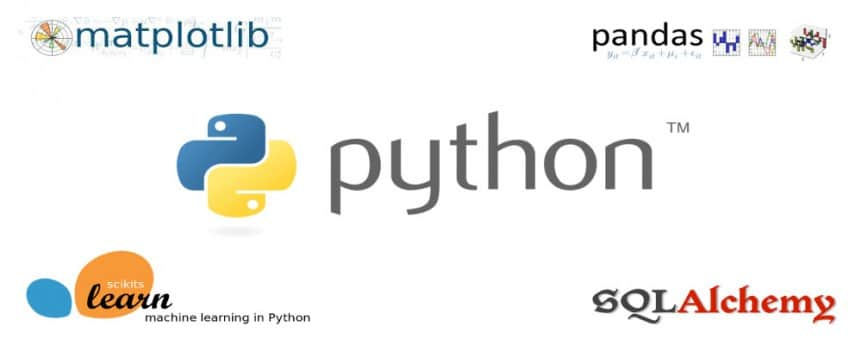
\includegraphics[width=300]{ghg.jpg}
\caption{librairies}
\end{center}
\end{figure}

\newpage
\subsection{DataSet}
Un DataSet, pour résumer, est une représentation d'une base de données sous forme d'objet. Il contient des tables, elles-mêmes contiennent des colonnes et des lignes. On pourrait le schématiser par la figure suivante.
\begin{figure}[h]
\begin{center}
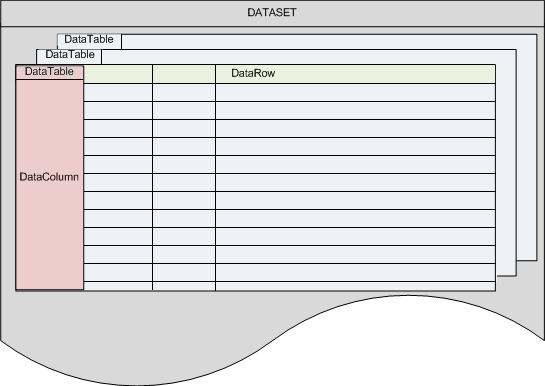
\includegraphics[width=300]{dataSet.png}
\caption{Schéma d'un DataSet}

\end{center}

\end{figure}
\subsection{La lecture de données}
Au niveau de notre projet l'ensemble données (DataSet) représente un fichier CSV qui contient l'ensemble des molécule et descripteur (Smille canonic) avec leur activité biologique sous nom (Observed) ,aussi plusieur autre colonne comme le nom de la molécule et rdkit Mol.
Pour apprendre à lire nos données nous allons faisant appel à un bibliothèque spécifiées qui s'appelle panda, Cela vous permet de lire et traiter ce fichier un enregistrement à la fois.

\newpage
\subsection{Concaténer les lignes et les colonnes}
après la lecture de données on passe par une étape très importante qui va nous faire concaténer les lignes et les colonnes, pour former de nouvelles structure de données \cite{ref25}.\\
\begin{table}[h]
\begin{center}
\begin{tabular}{|c|c|c|c|}
\hline
Row & Name & SmilesCanonical & Observed \\
\hline 
0 & Benzyl & Cc1ccccc1N & -0.36\\
1 & Aniline & N#CCc1ccccc1 & -0.24\\
2 & Benzane & CCc1cccc(N)c1 & 0.12\\
3 & Methilany & OCC=Cc1ccccc1 & 0.28\\
\hline
\end{tabular}
\caption{Concaténation entre trois colonnes}
\end{center}
\end{table}
\subsection{Transformation des données}
Les réseaux de neurones ne fonctionnent pas directement sur les cadres de données Python. Un réseau de neurones nécessite une matrice \textbf{numérique} ou format numérique. pour convertir les colonnes qui ne sont pas au format numérique par exemple dans notre dataSet la colonnes de  SmilesCanonical est une format de chaine de caractère (String). \\
\begin{figure}[h]
\begin{center}
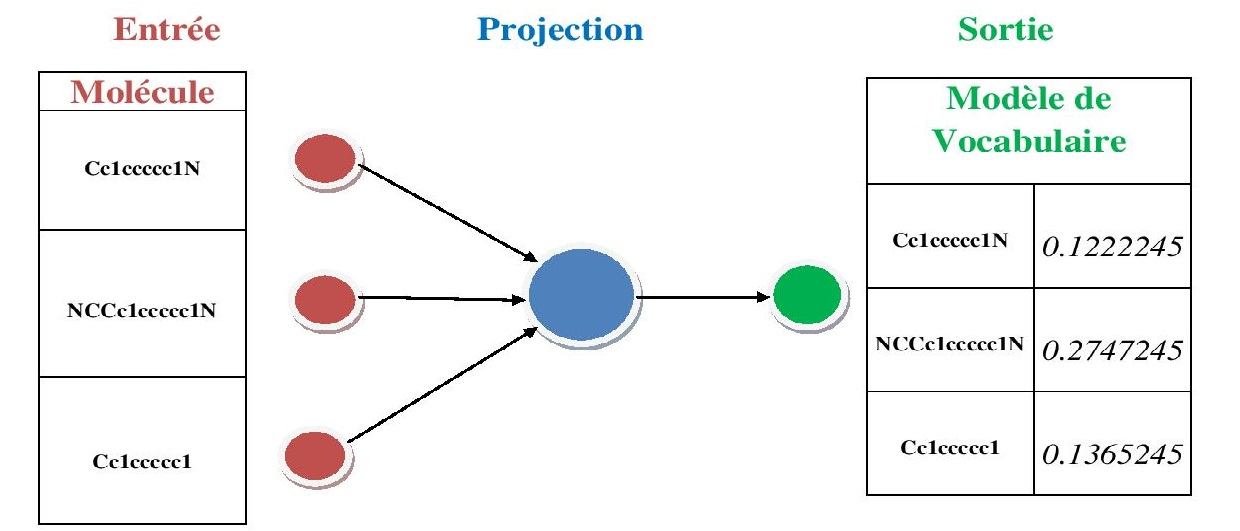
\includegraphics[width=340]{nlp.jpg}
\caption{Modèle de transformation}
\end{center}

\end{figure}



Alors on va utilisé des méthodes basés sur Le traitement du langage naturel NLP. pour trouvées un modèle puissante de transformation de format string vers le format numérique.

\subsubsection{Traitement automatique du langage naturel NLP}
est une branche très importante du Apprentissage automatique et donc de l'intelligence artificielle. Le NLP est la capacité d'un programme à comprendre le langage humain. Certains exemples pratiques de la NLP sont la reconnaissance vocale \cite{ref26}.

\begin{figure}[h]
\begin{center}
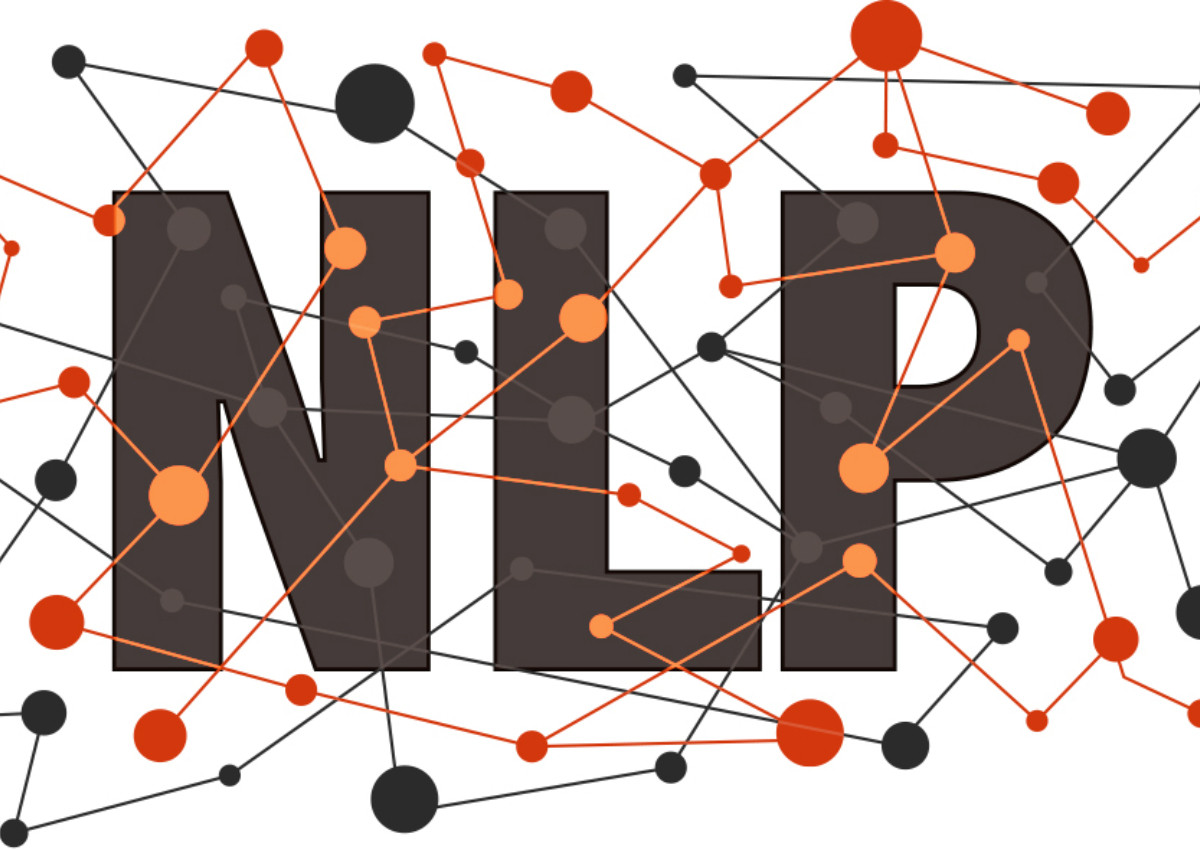
\includegraphics[width=150]{nnnp.jpg}
\caption{Langage naturel}
\end{center}



\end{figure}


\subsubsection{Transformation mot à vecteur word2vec}
est une structure de réseau de neurones permettant de générer l'intégration de mots en formant le modèle à un problème de classification supervisée. Une telle méthode a été introduite pour la première fois dans le document Estimation efficace des représentations de mots dans l'espace vectoriel  comme vous avez  déja vue dans la figure de Modèle de transformation \cite{ref27}.

\newpage 
\subsection{Définis le modèle}
Au niveau d'une application d'apprentissage en profondeur ,L'étape la plus importante est de définir \textbf{le modèle} et leur \textbf{architecture} après de choisir le type de modèle, Alors on a choisi le type de modèle le plus  utilisé est le modèle \textbf{séquentiel} .\\
Un excellent moyen d'utiliser l'apprentissage en profondeur  consiste à créer un réseau de neurones à convolution (CNN). 
\begin{figure}[h]
\begin{center}
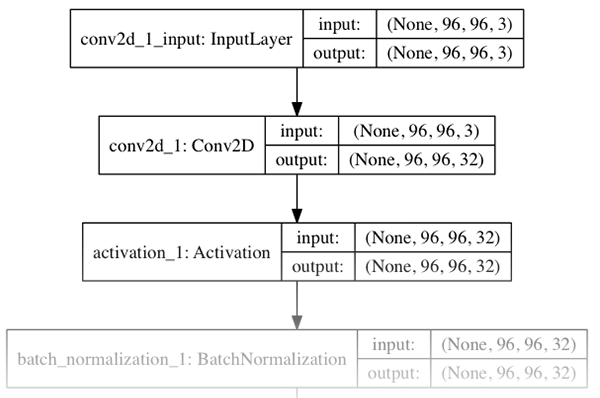
\includegraphics[width=300]{cnnmodel.png}
\caption{Modèle CNN}
\end{center}
\end{figure}

\subsubsection{Le modèle séquentiel}
Le modèle doit savoir à quelle forme d'entrée il doit s'attendre. Pour cette raison, la première couche d'un modèle séquentiel doit recevoir des informations sur sa forme en entrée \cite{ref29}.

\subsubsection{Spécifier la forme d'entrée}
Le modèle doit savoir à quelle forme d'entrée il doit s'attendre. Pour cette raison, la première couche d'un modèle séquentiel (et uniquement la première, car les couches suivantes peuvent effectuer une inférence de forme automatique) doit recevoir des informations sur la forme en entrée \cite{ref28} .\\ 
cette entrée Passez par un argument \textbf{inputshape} à la première couche.
\subsubsection{Définis le réseau de neurones}
Dans cette étape nous avons choisir le type de réseau de neurones quant va utilise dans notre modèle qui est 
le CNN. le réseau de neurones de convolution est similaire à un réseau de perceptrons multicouches. Les principales différences sont ce que le réseau apprend, comment il est structuré et à quoi il sert principalement \cite{ref30} .\\
\begin{figure}[h]
\begin{center}
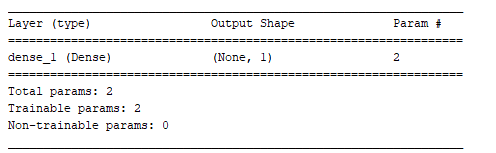
\includegraphics[width=300]{Capture.png}
\caption{Modèle CNN}
\end{center}
\end{figure}
\subsubsection{Le réseau de neurones de convolution Conv1D}
Cette couche crée un noyau de convolution qui est convolutionné avec l'entrée de couche sur une seule dimension spatiale (ou temporelle) pour produire un tenseur de sorties \cite{ref31} . par exemple :\\
\textcolor{red}{ keras.layers.Conv1D(filters, kernelsize, inputshape, activation='relu')} \cite{ref31}

\subsubsection{Le réseau de neurones de convolution Conv2D}
Cette couche crée un noyau de convolution qui est convolué avec l'entrée de la couche  sur une deux dimension pour produire un tenseur de sorties. dans notre modèle nous avons utilisé le Conv2D parce que notre vecteur de données est avec deux dimension \cite{ref31} . par exemple :  \\
\textcolor{red}{keras.layers.Conv2D(filters, kernelsize, inputshape, activation='relu')} \cite{ref31}
\newpage
\subsubsection{Les Arguments utilisé aux CNN}
généralement les arguments utilisé au niveaux de réseau de neurones de convolution :
\begin{enumerate}
\item \textbf{filtres :} la dimensionnalité de l'espace de sortie (c'est-à-dire le nombre de filtres de sortie dans la convolution).
\item \textbf{kernelsize:} liste d'un seul entier, spécifiant la longueur de la fenêtre de convolution 1D.
\item \textbf{Activation:} Les activations peuvent être utilisées via une couche d'activation ou via l'argument d'activation pris en charge par toutes les couches .
\end{enumerate}

\subsection{Mettre le modèle à l'entrainement sur les données}
Avant de passé le modèle à l'entrainement sur l'ensemble de données qui nous avons lire a partir \textbf{dataSet} vous devez configurer le processus d'apprentissage, qui s'effectue via la méthode de \textbf{compilation} \cite{ref31} , comme suit :\\
\textcolor{red}{model.compile(optimizer='rmsprop', loss='mse')} \cite{ref31}\\
après l'étape de compilation en passe directement à l'étape de l'entrainement sur l'ensemble de données ou qui 'il s'appelle l'ensemble d'apprentissage pour construire et évaluer le modèle de prédiction par une grand partie de notre données et lasse l'autre pour le test et l'évaluation \cite{ref25}. comme suit :\\
\textcolor{red}{model.fit(X ,Y,batchsize=1,epochs=100)} \cite{ref31}
\begin{figure}[h]
\begin{center}
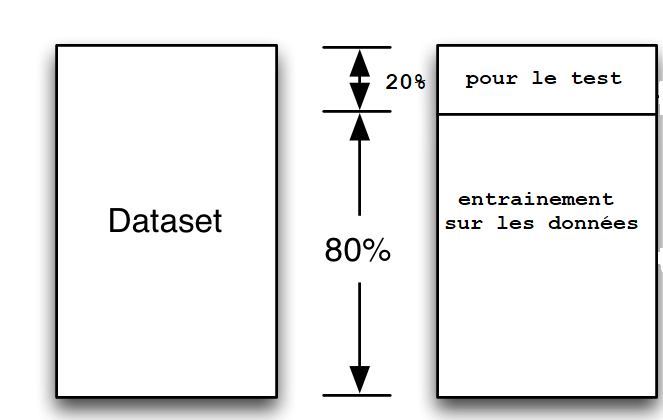
\includegraphics[width=200]{evalu2.png}
\caption{L'entrainement et l'évaluation sur les données}
\end{center}
\end{figure}

\subsection{La prédiction }
Après la phase de test nous atteindrons notre objectif consistant à établir un modèle d'apprentissage en profondeur basé sur un réseau de neurones convolutifs pour utilisé sur la modélisation Qsar pour la prédiction de l'activité biologique,enfin Génère des prédictions de sortie pour les échantillons d'entrée comme suit :\\
\textcolor{red}{predict(X, batchsize=None, verbose=0)} \cite{ref31}
\newpage
\section{Implémentation}
...
\newpage
\section{Les outils utilisés}
Au cours de cette étape, nous soulignerons les divers outils que nous avons utilisés pour mener à bien notre projet concerné l'apprentissage en profondeur pour la prédiction de l'activité biologique.
\subsection{Définition Pycharm }
\begin{multicols}

\includegraphics[width=100]{PyCharm.png}
PyCharm est un environnement de développement intégré utilisé pour programmer en Python.
Il permet D'analyse de code et contient un dèbogueur graphique. Il permet également la gestion des tests unitaires, l'intégration de logiciel de gestion de versions  \cite{ref32}.

\end{multicols}
\subsection{Pourquoi nous avons choisi Pycharm ? }
Dans PyCharm, nous pouvez voir où et comment sont définis les symboles, tels que les balises, les classes, les champs, les méthodes ou les fonctions, dans notre projet. À cette fin, l'IDE propose la fenêtre de définition rapide  \cite{ref32}.\\
Vu que l’API Python de TensorFlow est la plus complète, nous l'avons choisi pour travailler et donc c’est pour ça on a choisi Pycharm un environnement de développement dédié au langage Python.
\subsection{Définition Anaconda  }
\begin{multicols}

\includegraphics[width=100]{anaconda.png}
Anaconda est une distribution libre , des langages de programmation Python , appliqué au développement d'applications dédiées à la science des données et à l'apprentissage automatique (traitement de données à grande échelle, analyse prédictive, calcul scientifique)  \cite{ref34}.
\end{multicols}
\subsection{Pourquoi nous avons choisi Anaconda ? }
Anaconda est le moyen le plus simple d'exercer la science des données Python et l'apprentissage automatique sur Windows. Il s'agit du standard de l'industrie en matière de développement, de test et de formation sur un seul ordinateur  \cite{ref35}.
une distribution Python libre qui intègre directement un grand nombre de packages.
\subsection{Plateforme de développement (TensorFlow) }

\begin{center}
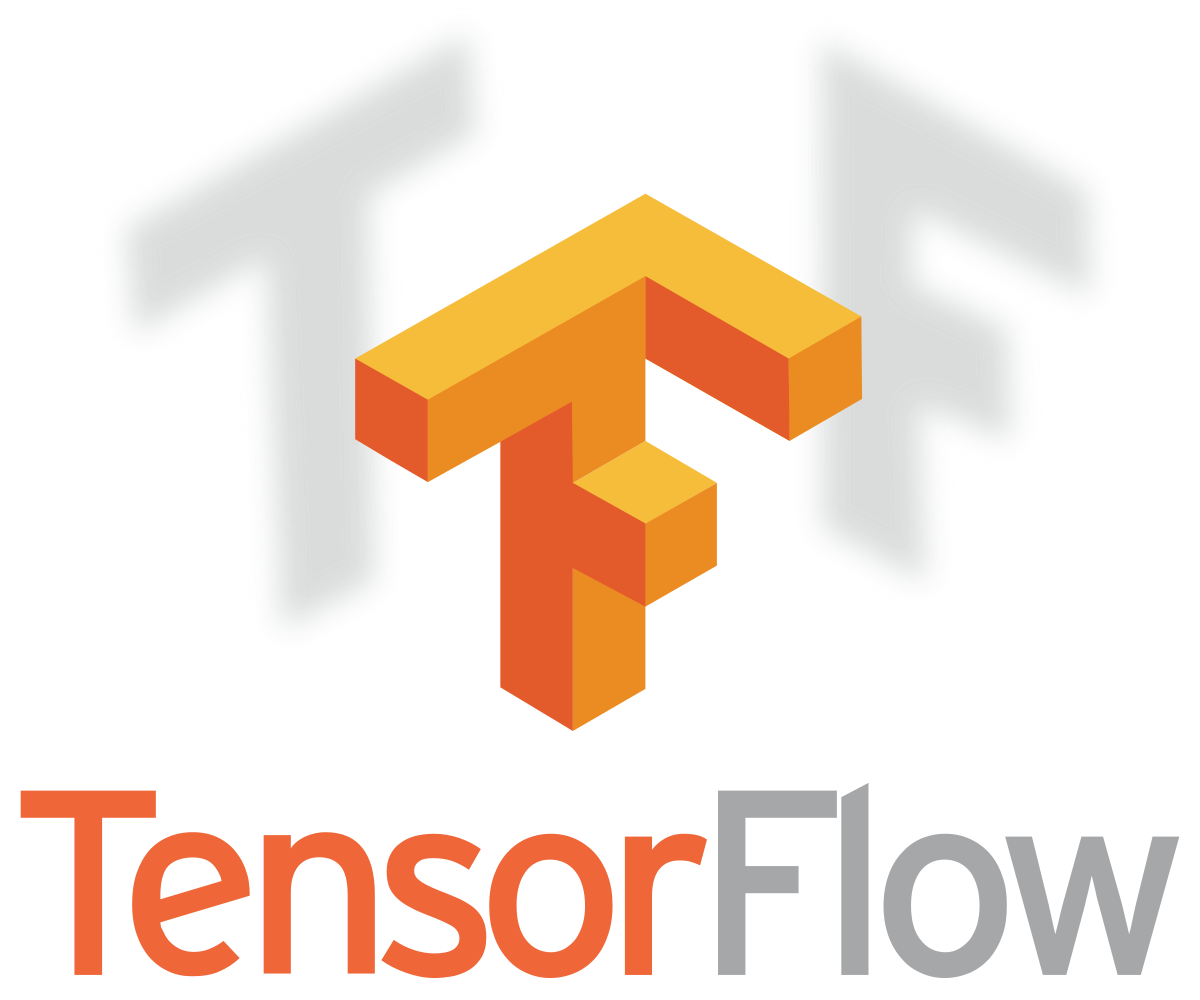
\includegraphics[width=100]{tonosr.png}
\end{center}


Nous avons utilisé dans notre travail TensorFlow qui est un framework de programmation pour le calcul numérique, développé par l'équipe Google Brain et qui a été rendu Open Source par Google en Novembre 2015. La version 1.0.0 a été lancée en février 2017  \cite{ref36}.
Depuis sa libération, TensorFlow n'a cessé de gagner en popularité, pour devenir très rapidement l'un des frameworks les plus utilisés pour le Deep Learning, comme le montrent les dernières comparaisons \cite{ref37}.\\
TensorFlow est très populaire pour ses nombreux avantages qu'on cite ci-dessous:
\begin{enumerate}
\item Multi-plateformes (Linux, Mac OS, et même Android et iOS ).
\item APIs en Python, C++, Java et Go (l’API Python est plus complète cependant, c’est sur celle-ci que nous allons travailler).
\item Temps de compilation très courts.
\item Supporte les calculs sur CPU, GPU et même le calcul distribué sur cluster.
\item Documentation extrêmement bien fournie avec de nombreux exemples et tutoriels.
\end{enumerate}
TensorFlow est aujourd'hui particulièrement utilisé pour l'apprentissage en profondeur, et donc les réseaux de neurones. Son nom est notamment inspiré du fait que les opérations courantes sur des réseaux de neurones sont principalement faites via des tables de données multi-dimensionnelles, appelées Tenseurs (Tensor). Un Tensor à deux dimensions est l'équivalent d’une matrice)  \cite{ref37}.\\
Aujourd'hui, les principaux produits de Google sont basés sur TensorFlow: Gmail, Google Photos, Reconnaissance de voix,….,etc.


\newpage
\bibliographystyle{plain}
\bibliography{bibc}


\end{document}
